\chapter{Electron-Ion Collider}\label{cha:EIC} % chktex 24

The Electron-Ion Collider (usually referred to by its abbreviation EIC) is a planned accelerator facility to be built at Brookhaven National Laboratory[cite BNL] in the place of today's Relativistic Heavy Ion Collider (known as RHIC). Contrary to RHIC, which was built as an ion-ion collider, EIC will open new possibilities of probing the structure of nucleons by colliding the comparably "simple-structured" electrons with the more complicated ions. Its versatile design will allow for a wide range of these ions – from protons (hydrogen ions) up to uranium [cite Silvia DIS].

\section{From RHIC to EIC}










% \section{Motivation...?}
% just an introduction, further explanations of the processes in cha:physics

% \section{Current Design Plan (from RHIC to EIC?)}

% \textit{the changes from usual illustrations (copied)}:\\
% In 2024, the project made several key EIC design decisions. They will lead to
% formal Project Scope changes after the Technical Change Control Board (TCCB)
% and the CCB processes.
% \begin{enumerate}[topsep=1mm, itemsep=0mm]
%     \item Reuse the entire Yellow RHIC ring, delay the 41-GeV bypass (a Blue RHIC arc).
%     \item Implement a new room-temperature Hadron Storage Ring (HSR) injection line.
%     \item Drop Strong Hadron Cooling (SHC), add Low-Energy Cooling (LEC).
%     \item Move the Rapid Cycling Synchrotron (RCS) out of the collider tunnel.
%     \item Delay the 28 nC/bunch and the 18 GeV capability implementation (ESR and RCS).
% \end{enumerate}
% These design decisions resolve uncertainties, challenges, and risks to EIC
% performance, safety, and future operation and maintenance. [Nagaitsev Frascati]


% maybe will fit better in another chapter

% \section{Advantages? \textit{Prínosy}}

% \section{Second detector?}
% is anyone seriously working on it, or is it too soon to care?

% maybe next to each other? - EIC should be still larger?
% \begin{figure}[H]
%     \centering
%     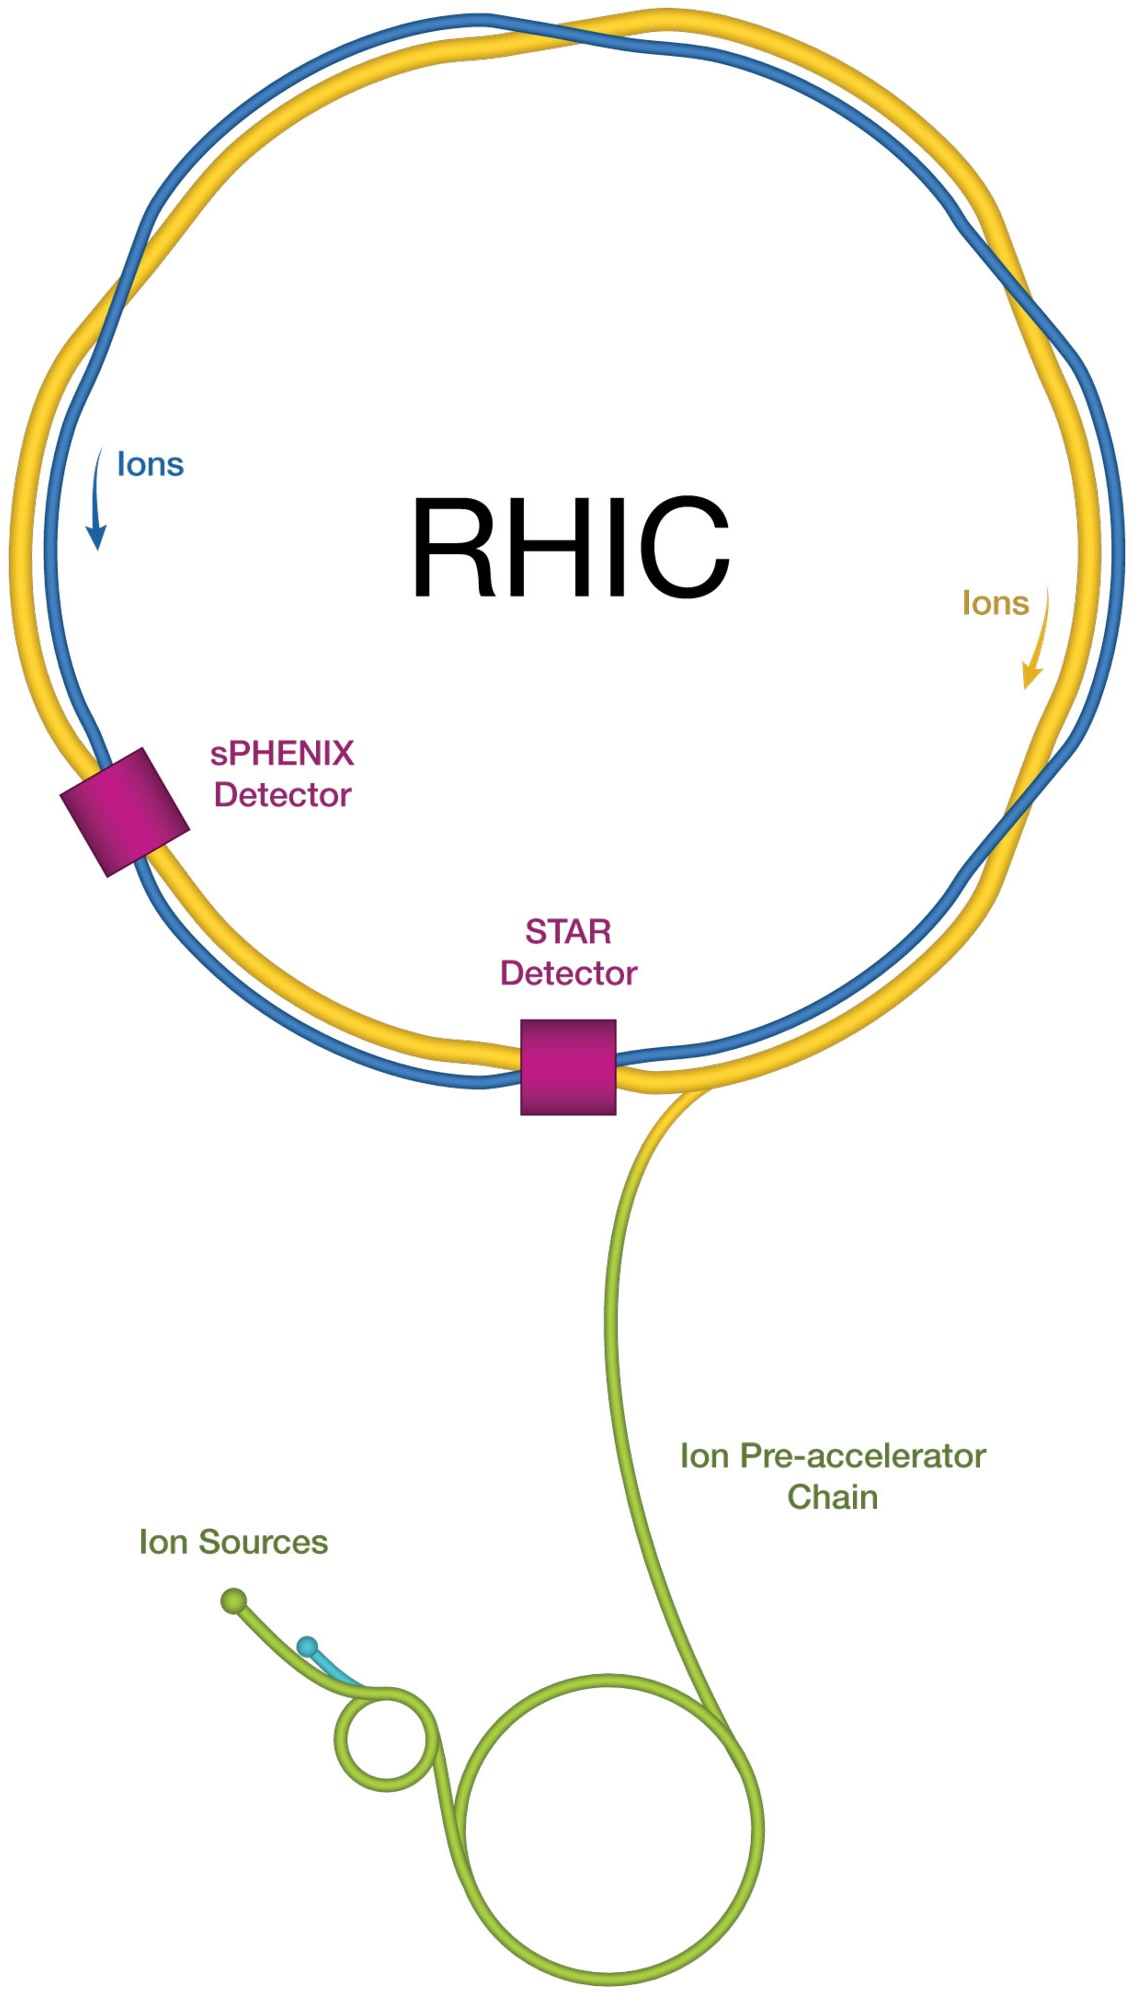
\includegraphics[width=.4\linewidth]{img/rhic.jpg}
%     \caption{\url{https://www.flickr.com/photos/brookhavenlab/51980309345/in/album-72157714316624996}}
%     \label{fig:eic:rhic}
% \end{figure}

% \begin{figure}[H]
%     \centering
%     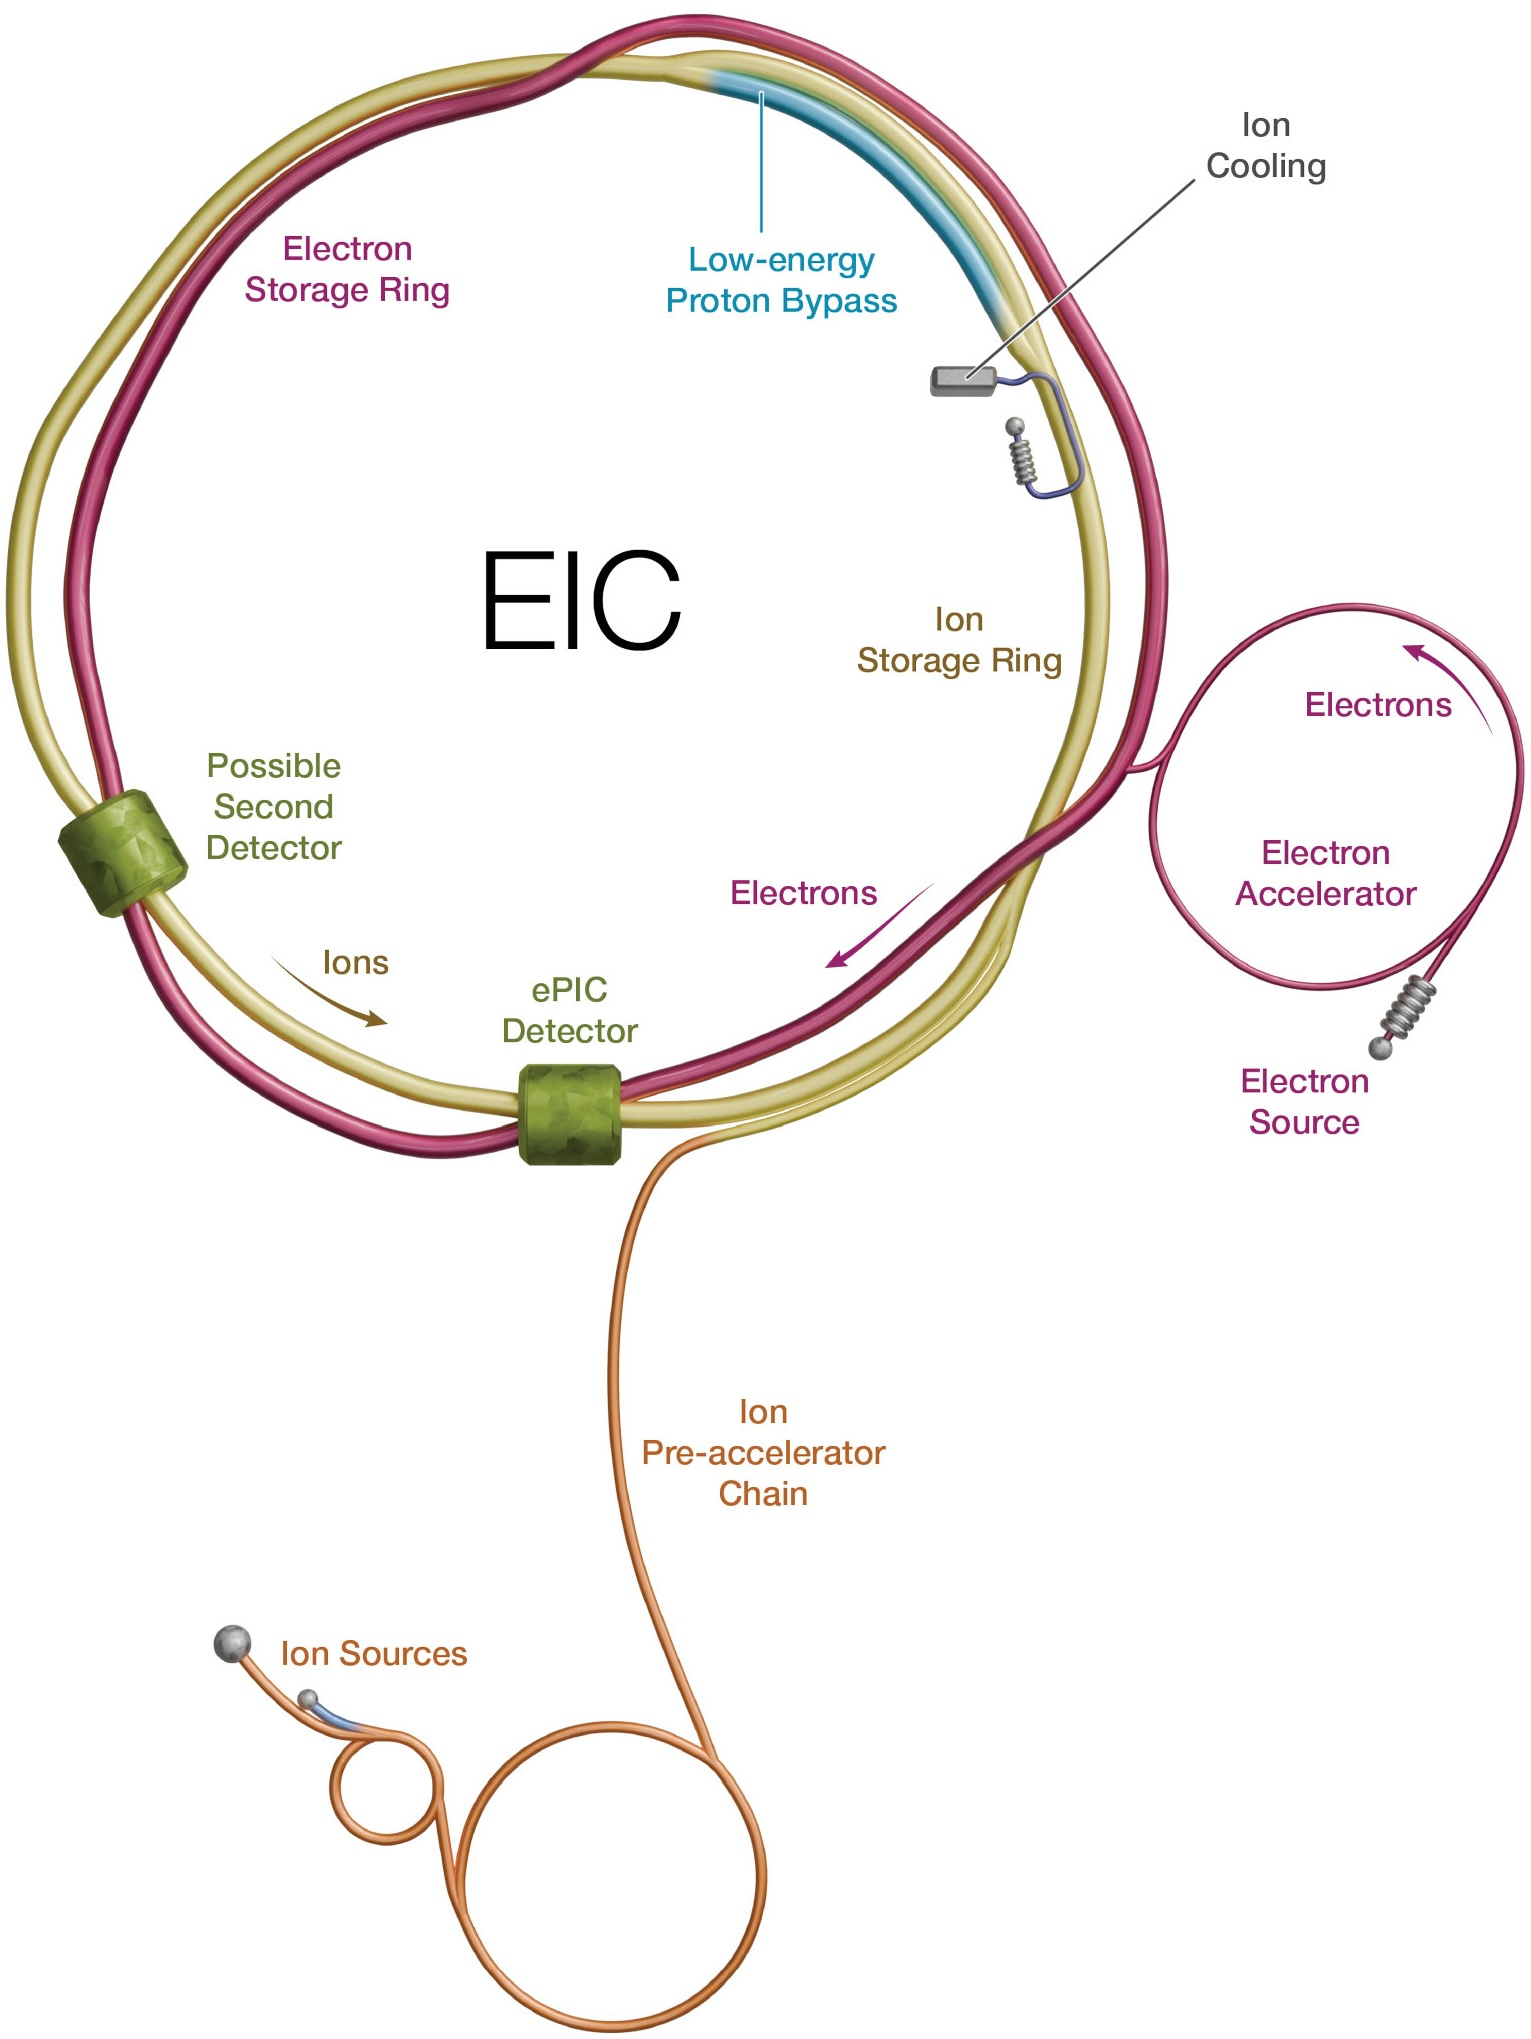
\includegraphics[width=.5\linewidth]{img/eic.jpg}
%     \caption{\url{https://www.flickr.com/photos/brookhavenlab/54007751967/in/album-72157714316624996}}
%     \label{fig:eic:eic}
% \end{figure}

% \begin{figure}[H]
%     \centering
%     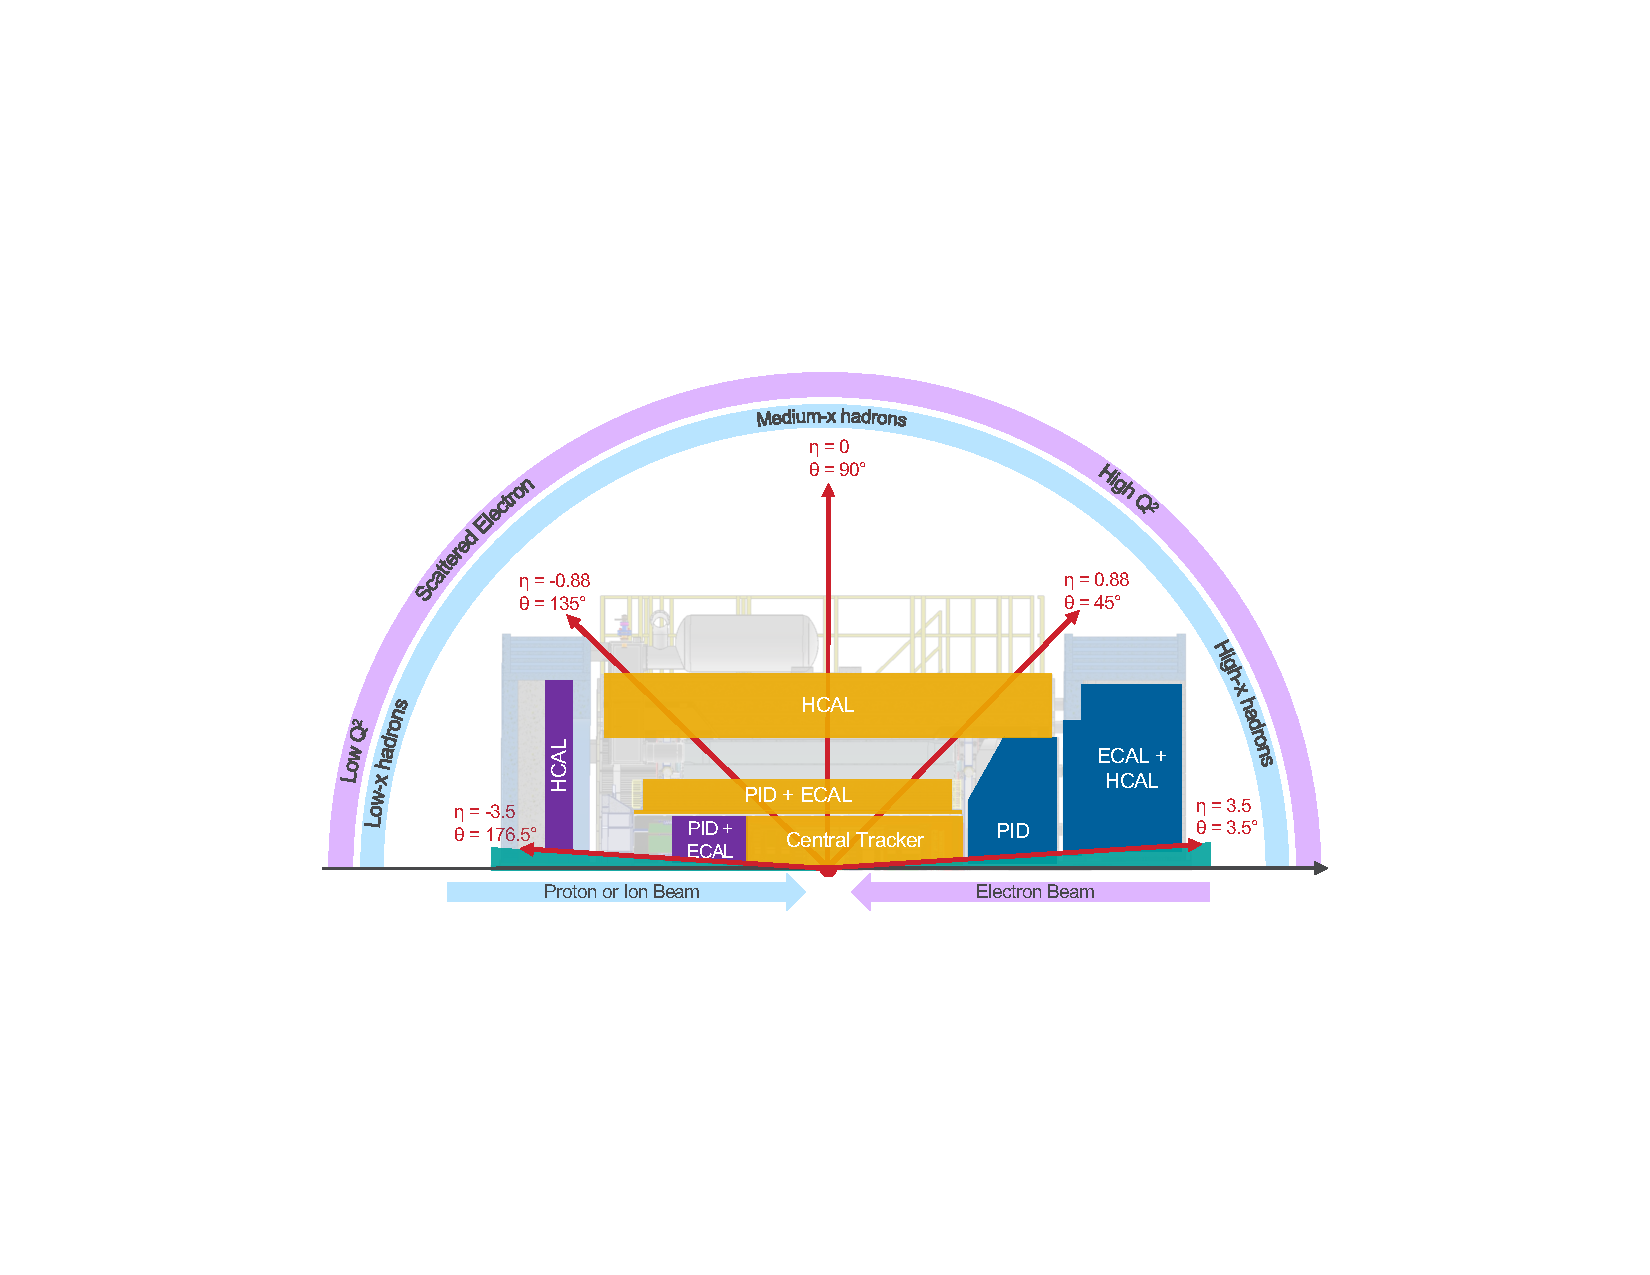
\includegraphics[width=.8\linewidth]{img/range.pdf}
%     \caption{always this image \url{https://doi.org/10.5281/zenodo.14939545}}
%     \label{fig:eic:range}
% \end{figure}